\documentclass[11pt,singlecolumn]{scrartcl}
\usepackage{amsmath,amssymb,amstext}
\usepackage[utf8]{inputenc}
\usepackage[english]{babel}
\usepackage{fancyhdr}
\usepackage{graphicx}
\usepackage[capposition=bottom]{floatrow}
\usepackage{listings}
\usepackage{float}

\begin{document}
\section{Hardware}
All the experiments were conducted on an ETH server (exact model?). This machine possesses 4 x 12 AMD Opteron 6174 processors, each one running at 2.2 GHz. The operating System was Debian 7.0 and the installed memory was 128 GB of RAM.
\section{Topologies}
In the experiment, four different topologies were used:\\\\
\textbf{Large Fattree} \quad  The large fattree topology is the largest one of the four topologies. It contains 55'000 vertices, of which 2'880 are switches. Furthermore the graph posses a total of 50'000 bidirectional edges. Since one bidirectional edge is represented by two directed edges, there are a total of 100'000 edges in the collection.\\\\
\textbf{Small Fattree} \quad The small fattree topology has the same vertices to edge ratio as the large fattree, but it is overall much smaller. It contains 17'665 vertices, of which 1'280 are switches. Furthermore the graph possesses a total of 16' 400 bidirectional edges. (needs better formulation) \\\\
\textbf{Large Jellyfish} \quad  The large jellyfish topology matches the large fattree in terms of vertices, but contains far less edges. It contains 56'160 vertices, of which 864 are switches. Furthermore the graph possesses a total of 6'910 bidirectional edges. (needs better formulation)\\\\
\textbf{Small Jellyfish} \quad The small jellyfish topology is the smallest one of the four topologies. It contains 16'770 vertices, of which 390 are switches. Furthermore the graph possesses a total of 2'145 bidirectional edges. (needs better formulation)
\section{Expectations}
In all topologies, weight is an attribute of the edges and uniformly distributed from 1 to 9. Consequently, the selection 'weight < 2' will therefore remove around 89\% of all edges. A lesser amount of edges immensely shortens the duration of any subsequent join process.\\ Since joining the entire vertex and edge set is a very costly operation, it is possible that queries with multiple, but restricted joins are faster than such, which contain fewer joins, but do not include any restrictions on the edge set. \\\\
Furthermore, it is important to consider the fact that the attributes of vertices and edges in a Differential Dataflow Collection are stored in a Vector of (String, Literal) tuples. We chose this suboptimal implementation since Differential Dataflow does not aprreciate HashMaps at all. However, in order to do a selection on either set, this Vector has to be transformed back into a HashMap for each edge respectively vertex. This process can be quite timeconsuming, therefore the more selection a query contains, the slower it expected to be.\\\\
It should also be noted that one single edge in the query triggers two joins in the evaluation. Reason being that we have to join the edge collection twice with the vertex collection, in order to determine all adjacent vertices of a given vertex.\\\\\\
In total, we ran seven different queries, with each subsequent query being more complex than the preceding one. For each query the resulting dataflow is drawn on the following pages. The numbers on the edges indicate the size of (intermediate) result set on the large fattree.\clearpage
\section{Overview}
\begin{figure}[H]
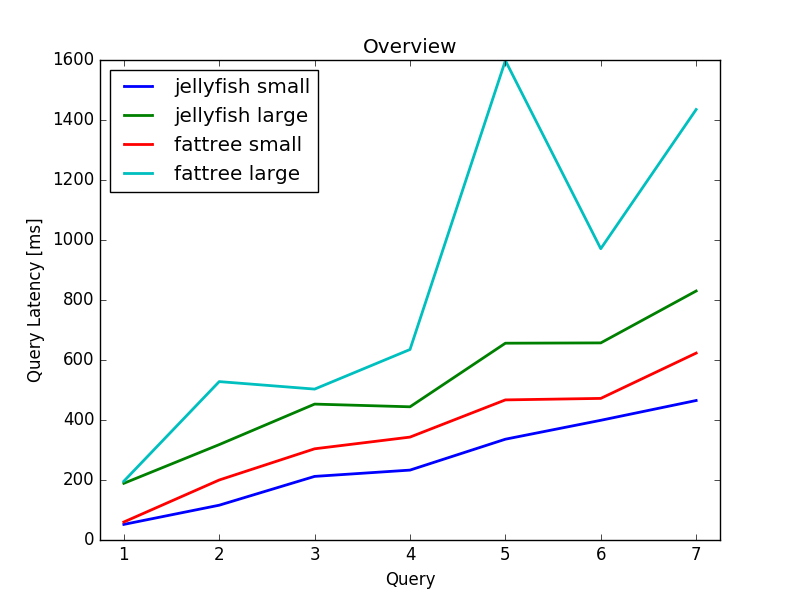
\includegraphics[width=1\textwidth]{ov}
\caption{An overview of the seven queries, run with 32 workers}
\end{figure}
Throughout all seven queries, the following pattern is noticeable:\\
The influence of the number of workers behaves unexpectedly, especially for queries 1,4 and 6. In a perfect world, the query latency would be inversely proportionalto the number of workers. However, we only observe this behaviour for query 5, and only for the fattree topologies.\\More often than not, an increase of worker threads leads to a higher latency, especially when the latency is already quite low, around the 50 to 200 millisecond range. We reason this happens because at that level, the communication overhead dominates the time savings achieved by parallelism. This is claim is additionally supported by the fact, that query 5 has one of the longest latencies, ranging up to 10 seconds. When evaluating queries with lower latency, the contention between the workers increases and we frequently observe that the best performance is achieved when running the query with just a single worker.\\
The following pages contain detailed boxplots and the dataflows for each of the seven queries.

\clearpage

\section{Query 1}
\begin{verbatim}
SELECT u.name WHERE u.label() = 'switch', u.position = 'access'
\end{verbatim}

\textbf{Peak Memory: 377'840 kb}\\
\textbf{Result size: 1'152} \\
2 simple selections, 0 joins. One pass through the vertices collection is enough to produce the result.\\\\
\textbf{Dataflow}
\begin{figure}[H]
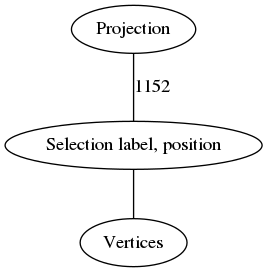
\includegraphics[width=0.4\textwidth]{graph1}
\caption{Dataflow Query1}
\end{figure}
\clearpage
\begin{figure}[!tbp]
  \centering
  \RawFloats
  \begin{minipage}[b]{0.5\textwidth}
    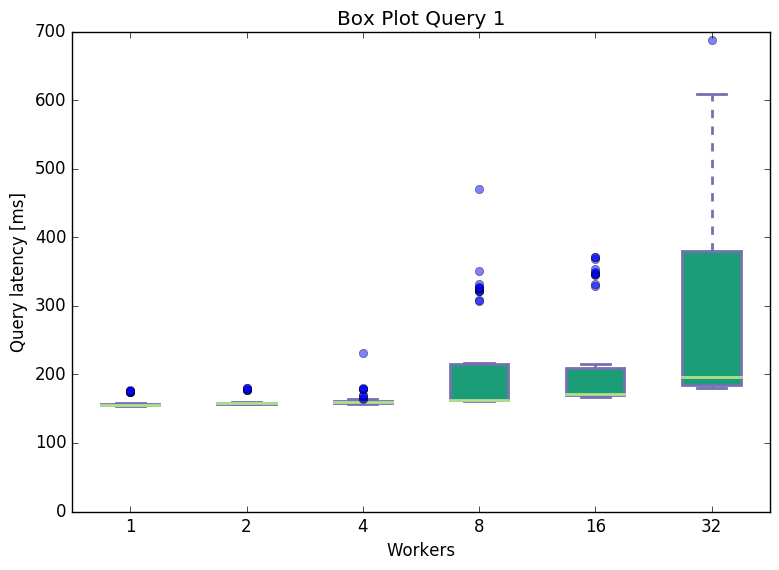
\includegraphics[width=\textwidth]{boxesfl/q1}
    \captionof{figure}{Large Fattree}
  \end{minipage}
  \hfill
  \begin{minipage}[b]{0.5\textwidth}
    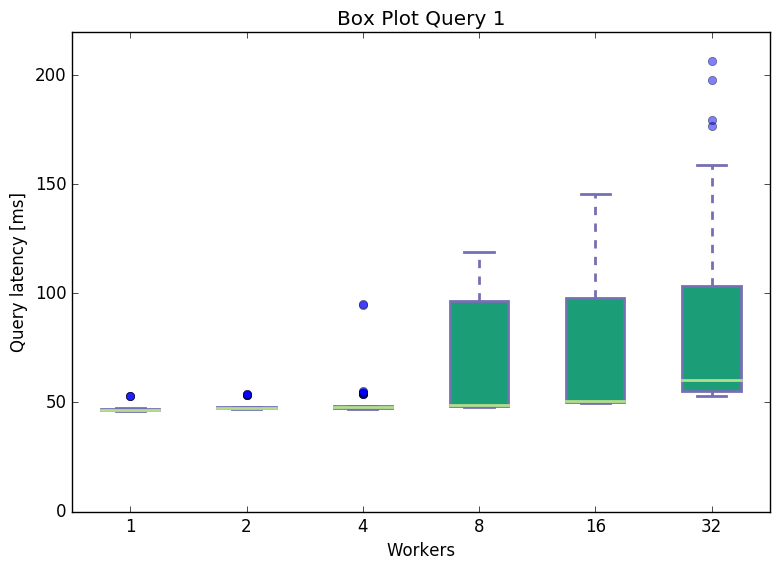
\includegraphics[width=\textwidth]{boxesfs/q1}
    \captionof{figure}{Small Fattree}
  \end{minipage}
\end{figure}
\begin{figure}[!tbp]
  \centering
  \RawFloats
  \begin{minipage}[b]{0.5\textwidth}
    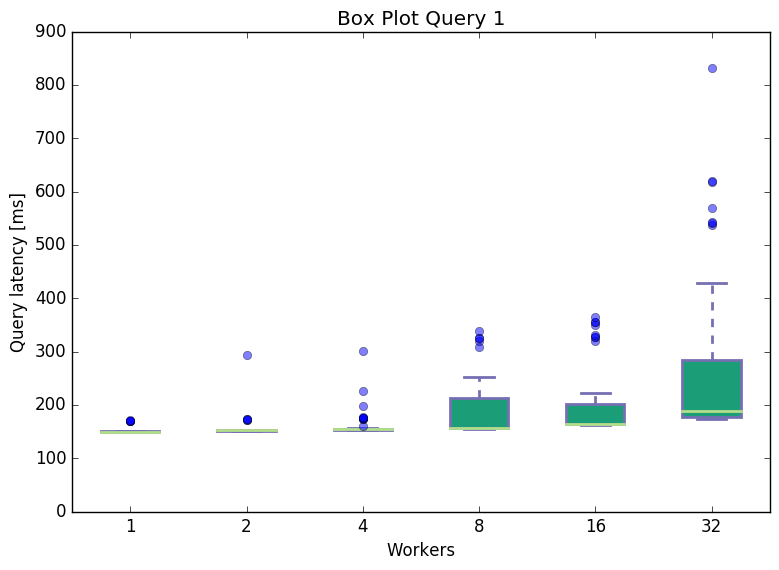
\includegraphics[width=\textwidth]{boxesjl/q1}
    \captionof{figure}{Large Jellyfish}
  \end{minipage}
  \hfill
  \begin{minipage}[b]{0.5\textwidth}
    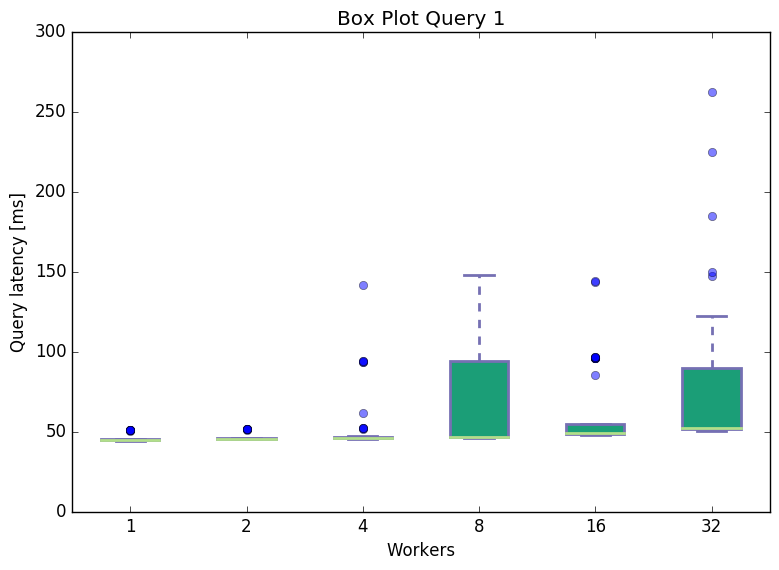
\includegraphics[width=\textwidth]{boxesjs/q1}
    \captionof{figure}{Small Jellyfish}
  \end{minipage}
\end{figure}
\clearpage
\section{Query2}
\begin{verbatim}
SELECT n.name WHERE (n) -[e with weight < 4]-> (m)\end{verbatim}

\textbf{Peak Memory: 3'597'452 kb}\\
\textbf{Result size: 36'542}\\
2 Joins and 1 Selection. The joins are not very expensive since we only use about 30\% of the edges.\\\\
\textbf{Dataflow}
\begin{figure}[H]
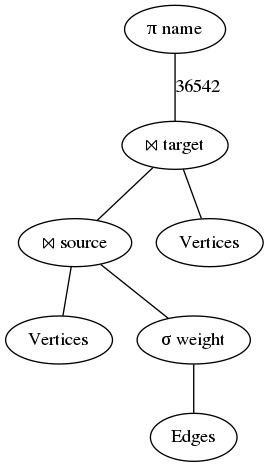
\includegraphics[width=0.4\textwidth]{graph2}
\caption{Dataflow Query2}
\end{figure}
\clearpage
\begin{figure}[!tbp]
  \centering
  \RawFloats
  \begin{minipage}[b]{0.5\textwidth}
    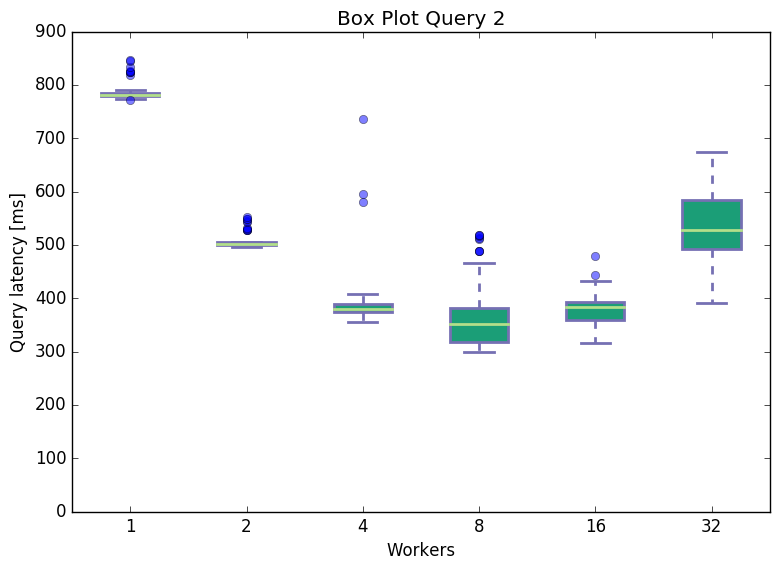
\includegraphics[width=\textwidth]{boxesfl/q2}
    \captionof{figure}{Large Fattree}
  \end{minipage}
  \hfill
  \begin{minipage}[b]{0.5\textwidth}
    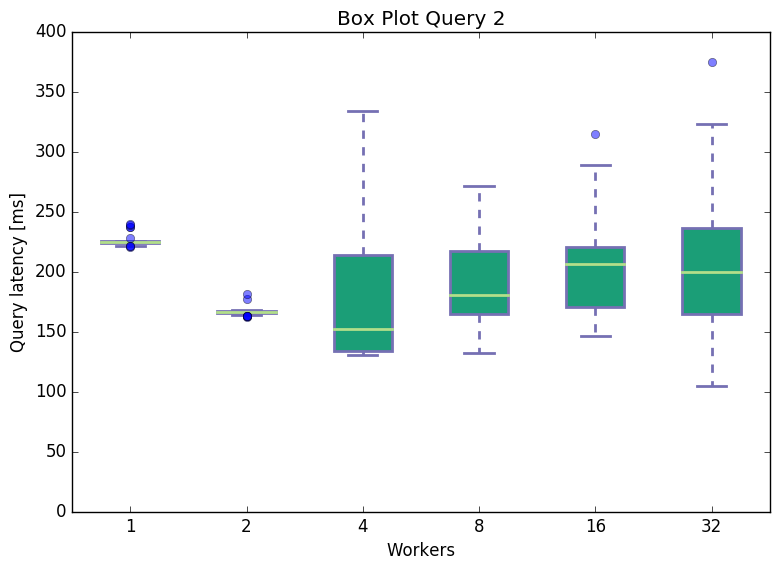
\includegraphics[width=\textwidth]{boxesfs/q2}
    \captionof{figure}{Small Fattree}
  \end{minipage}
\end{figure}
\begin{figure}[!tbp]
  \centering
  \RawFloats
  \begin{minipage}[b]{0.5\textwidth}
    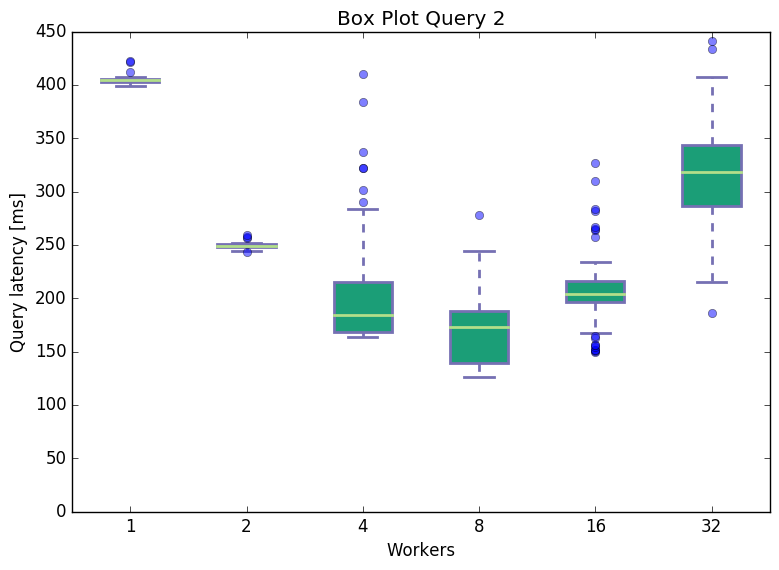
\includegraphics[width=\textwidth]{boxesjl/q2}
    \captionof{figure}{Large Jellyfish}
  \end{minipage}
  \hfill
  \begin{minipage}[b]{0.5\textwidth}
    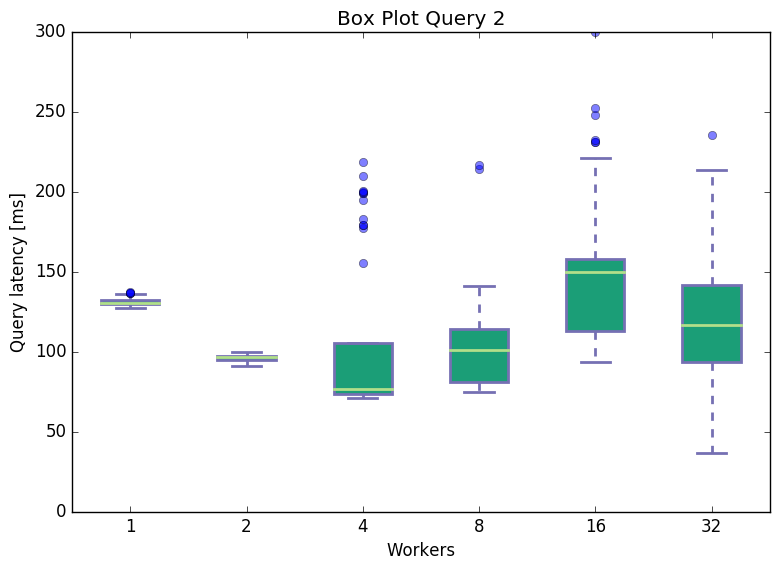
\includegraphics[width=\textwidth]{boxesjs/q2}
    \captionof{figure}{Small Jellyfish}
  \end{minipage}
\end{figure}
\clearpage
\section{Query3}
\begin{verbatim}
SELECT n.name WHERE (n:switch) -> (m with position = 'distribution')\end{verbatim}

\textbf{Peak Memory: 1'433'376 kb}\\
\textbf{Result size: 55'296}\\
2 Joins and 2 Selections. I expected this query to be a little bit slower since we are using all the edges in the joins, but it is only a tiny bit slower than Query 2.\\\\
\textbf{Dataflow}
\begin{figure}[H]
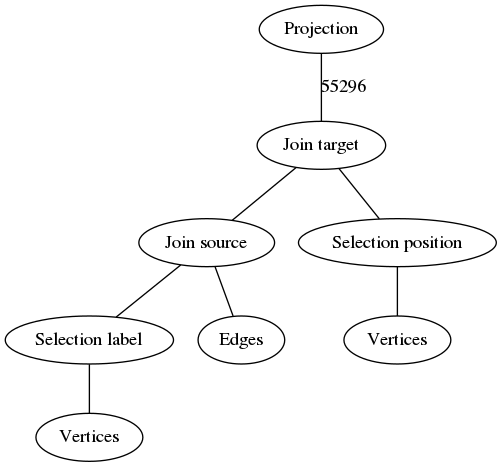
\includegraphics[width=0.6\textwidth]{graph3}
\caption{Dataflow Query3}
\end{figure}
\clearpage
\begin{figure}[!tbp]
  \centering
  \RawFloats
  \begin{minipage}[b]{0.5\textwidth}
    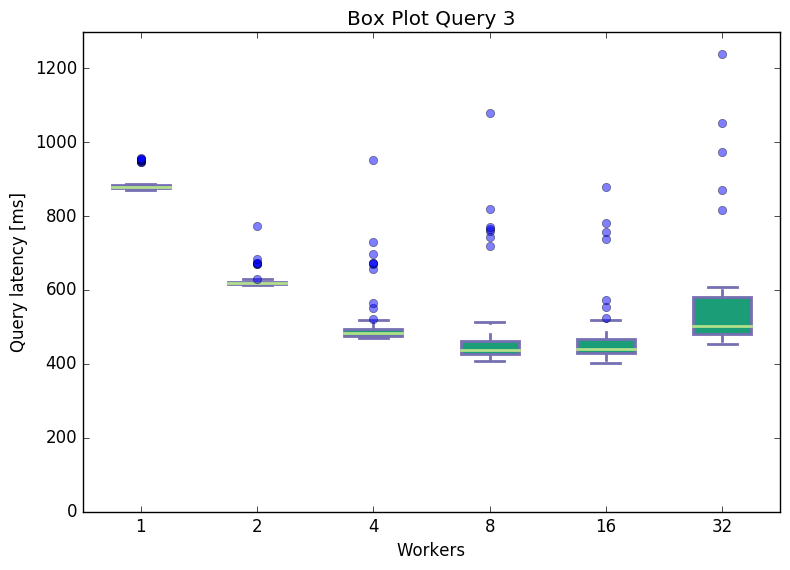
\includegraphics[width=\textwidth]{boxesfl/q3}
    \captionof{figure}{Large Fattree}
  \end{minipage}
  \hfill
  \begin{minipage}[b]{0.5\textwidth}
    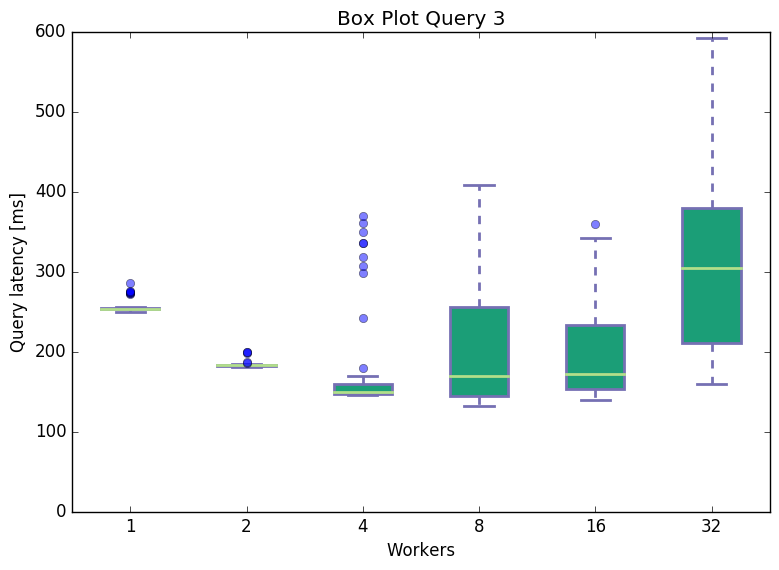
\includegraphics[width=\textwidth]{boxesfs/q3}
    \captionof{figure}{Small Fattree}
  \end{minipage}
\end{figure}
\begin{figure}[!tbp]
  \centering
  \RawFloats
  \begin{minipage}[b]{0.5\textwidth}
    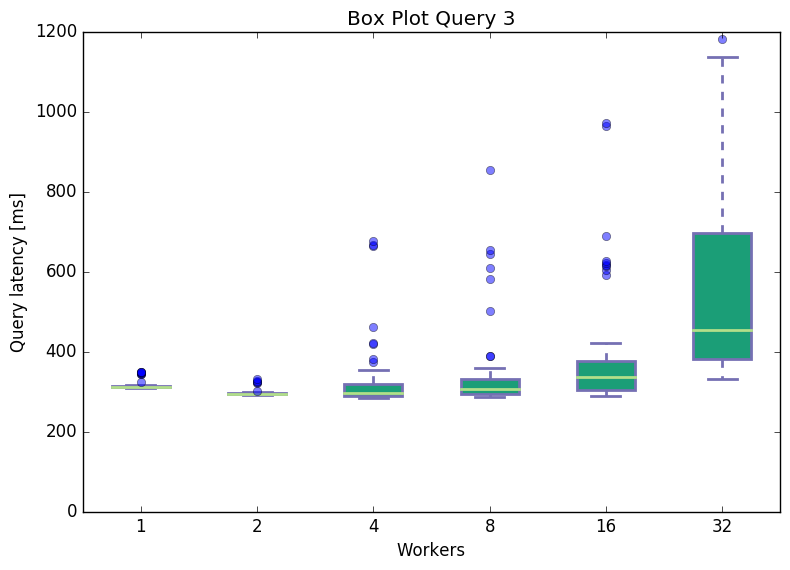
\includegraphics[width=\textwidth]{boxesjl/q3}
    \captionof{figure}{Large Jellyfish}
  \end{minipage}
  \hfill
  \begin{minipage}[b]{0.5\textwidth}
    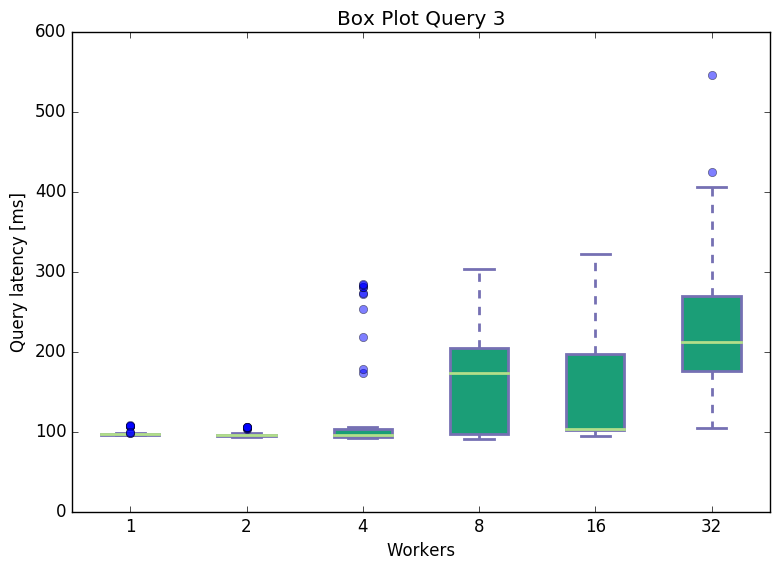
\includegraphics[width=\textwidth]{boxesjs/q3}
    \captionof{figure}{Small Jellyfish}
  \end{minipage}
\end{figure}
\clearpage
\section{Query4}
\begin{verbatim}
SELECT n.name WHERE (n with position = 'distribution')
-[e with weight > 8]-> (m with position = 'access')\end{verbatim}

\textbf{Peak Memory: 1'114'896 kb}\\
\textbf{Result size: 3'097}\\
2 Joins and 3 Selections. Even though this query has more constraints than Query 2 and 3, it is faster since we only use 10\% of the edges in the joins. \\\\
\textbf{Dataflow}
\begin{figure}[H]
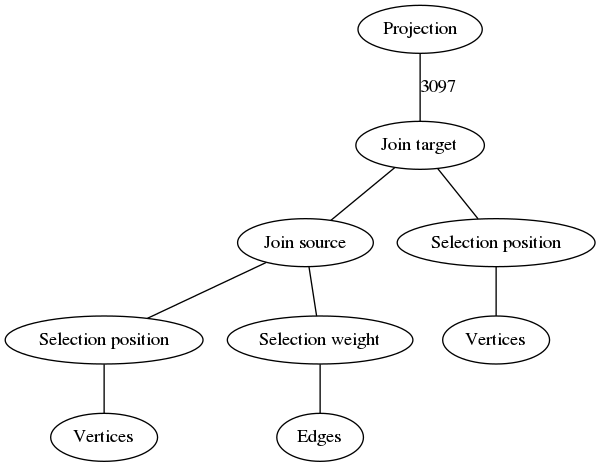
\includegraphics[width=0.6\textwidth]{graph4}
\caption{Dataflow Query4}
\end{figure}
\clearpage
\begin{figure}[!tbp]
  \centering
  \RawFloats
  \begin{minipage}[b]{0.5\textwidth}
    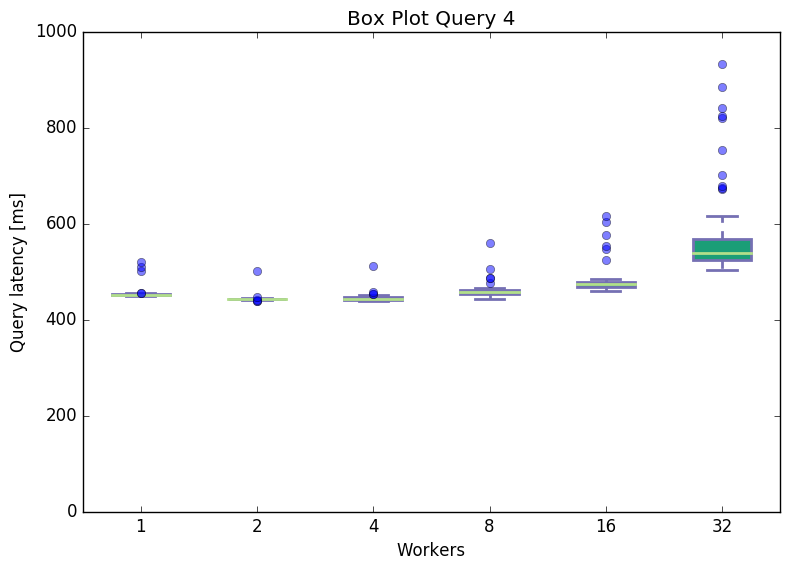
\includegraphics[width=\textwidth]{boxesfl/q4}
    \captionof{figure}{Large Fattree}
  \end{minipage}
  \hfill
  \begin{minipage}[b]{0.5\textwidth}
    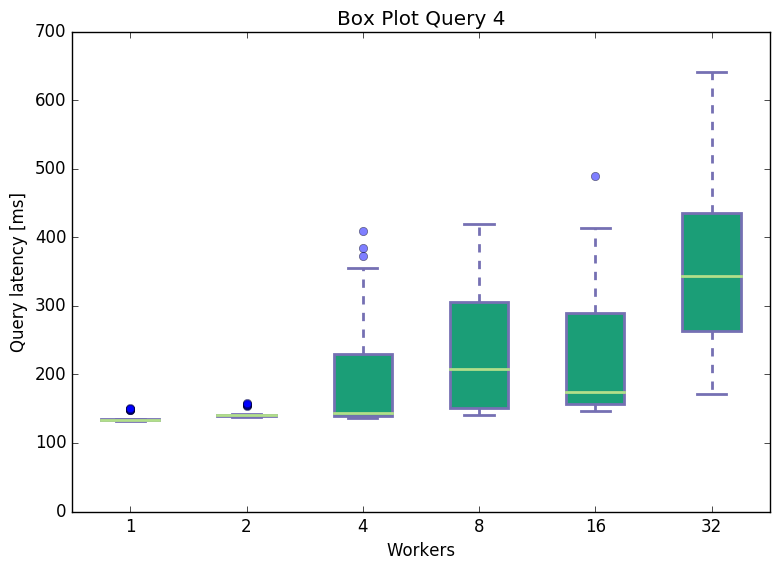
\includegraphics[width=\textwidth]{boxesfs/q4}
    \captionof{figure}{Small Fattree}
  \end{minipage}
\end{figure}
\begin{figure}[!tbp]
  \centering
  \RawFloats
  \begin{minipage}[b]{0.5\textwidth}
    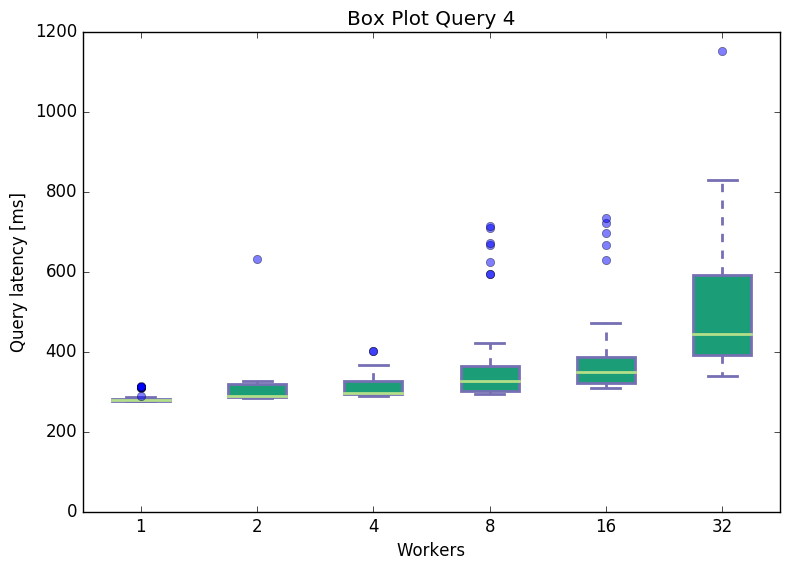
\includegraphics[width=\textwidth]{boxesjl/q4}
    \captionof{figure}{Large Jellyfish}
  \end{minipage}
  \hfill
  \begin{minipage}[b]{0.5\textwidth}
    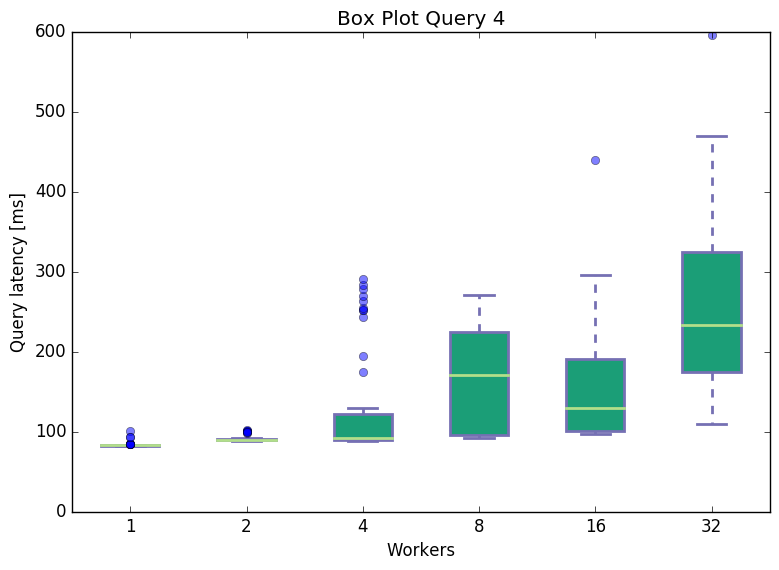
\includegraphics[width=\textwidth]{boxesjs/q4}
    \captionof{figure}{Small Jellyfish}
  \end{minipage}
\end{figure}
\clearpage

\section{Query5}
\begin{verbatim}
SELECT v.name WHERE (u WITH position = 'access')
 -> (v WITH position = 'distribution')
 -> (w WITH position = 'core')\end{verbatim}
\textbf{Peak Memory: 3'797'976 kb}\\
\textbf{Result size: 663'552}\\
4 Joins and 3 Selections. The last 3 queries all contain multiple query edges and are much slower. Since there is no selection on the edge, this particular query is quite slow even though it has "only" 4 joins.\\\\
\textbf{Dataflow}
\begin{figure}[H]
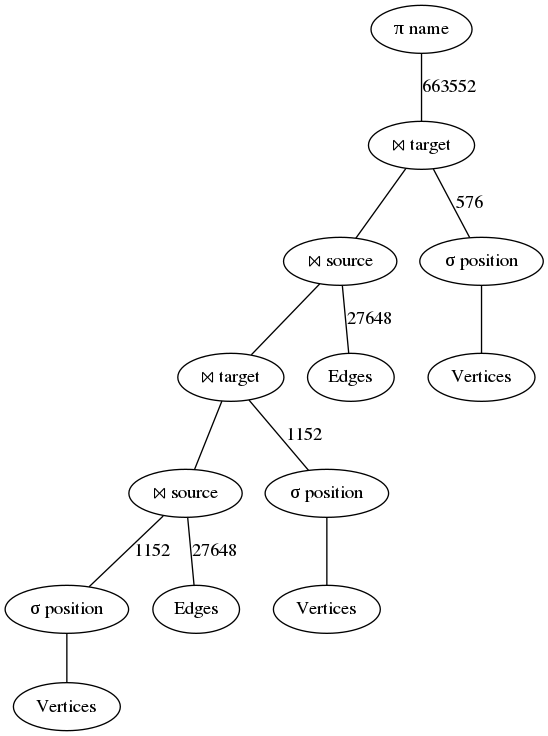
\includegraphics[width=0.6\textwidth]{graph5}
\caption{Dataflow Query5}
\end{figure}
\clearpage
\begin{figure}[!tbp]
  \centering
  \RawFloats
  \begin{minipage}[b]{0.5\textwidth}
    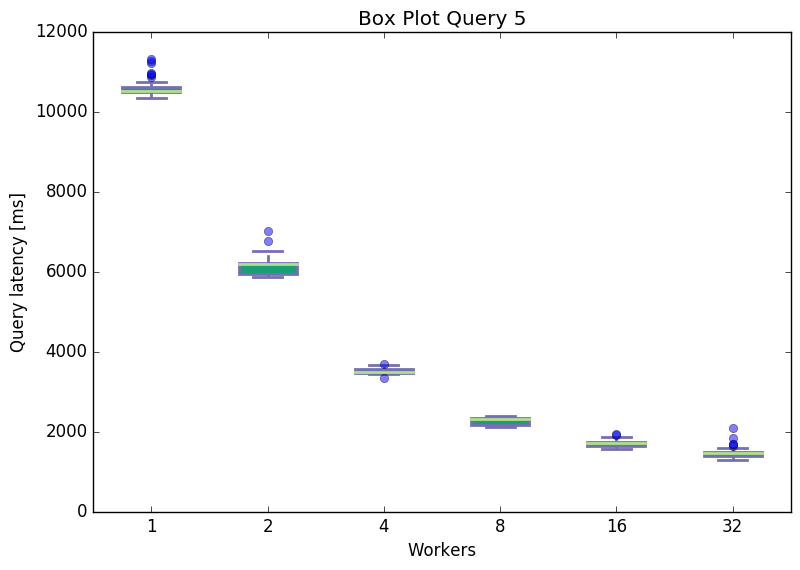
\includegraphics[width=\textwidth]{boxesfl/q5}
    \captionof{figure}{Large Fattree}
  \end{minipage}
  \hfill
  \begin{minipage}[b]{0.5\textwidth}
    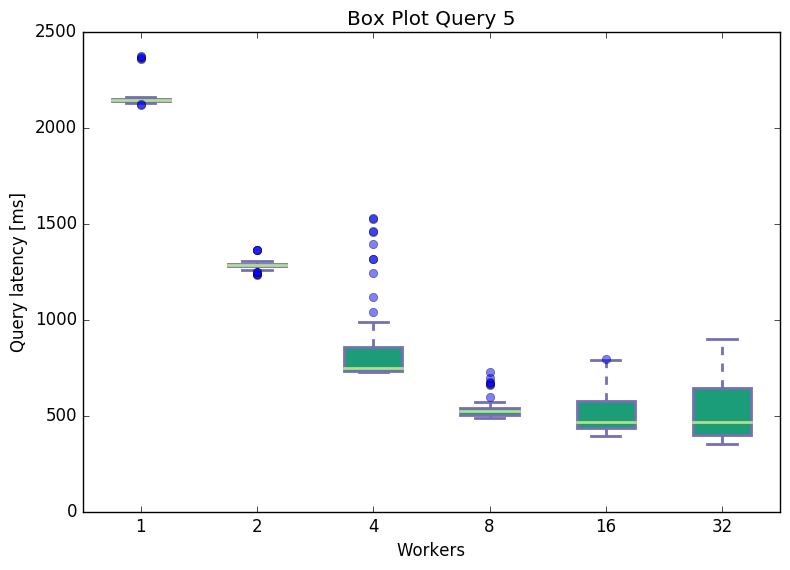
\includegraphics[width=\textwidth]{boxesfs/q5}
    \captionof{figure}{Small Fattree}
  \end{minipage}
\end{figure}
\begin{figure}[!tbp]
  \centering
  \RawFloats
  \begin{minipage}[b]{0.5\textwidth}
    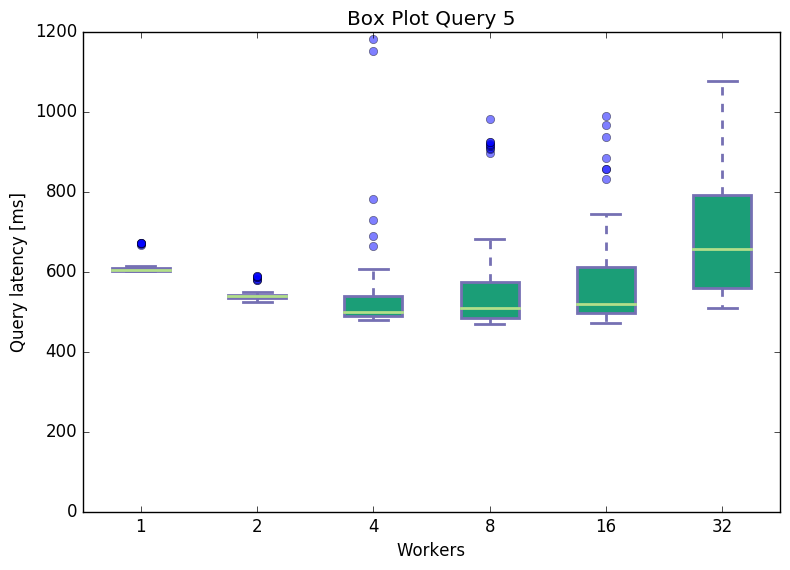
\includegraphics[width=\textwidth]{boxesjl/q5}
    \captionof{figure}{Large Jellyfish}
  \end{minipage}
  \hfill
  \begin{minipage}[b]{0.5\textwidth}
    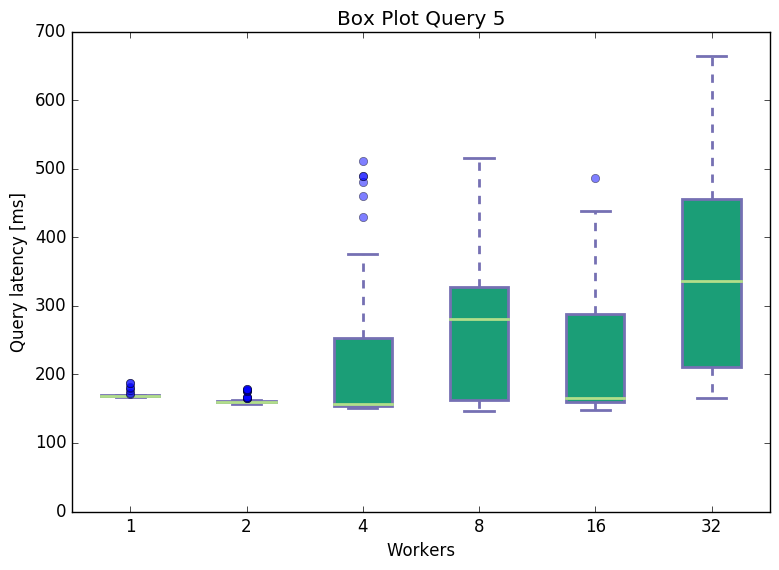
\includegraphics[width=\textwidth]{boxesjs/q5}
    \captionof{figure}{Small Jellyfish}
  \end{minipage}
\end{figure}
\clearpage

\section{Query6}
\begin{verbatim}
SELECT v.name WHERE (u WITH position = 'access')
 -[e with weight  < 2]-> (v WITH position = 'distribution')
 -[f with weight > 8]-> (w WITH position = 'core')\end{verbatim}
\textbf{Peak Memory: 1'573'940 kb}\\
\textbf{Result size: 8'334}\\
4 Joins and 5 Selections. Like query 4, the evaluation time goes down as we add more constraints on the edges. Since we have a lot less tuples in the 3rd and 4th join, this query is faster than previous one.\\\\
\textbf{Dataflow}
\begin{figure}[H]
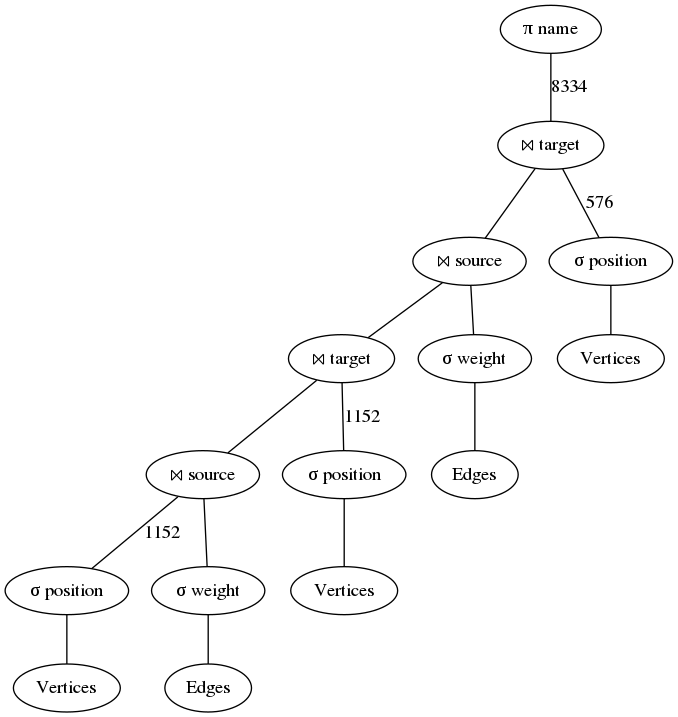
\includegraphics[width=0.8\textwidth]{graph6}
\caption{Dataflow Query6}
\end{figure}
\clearpage
\begin{figure}[!tbp]
  \centering
  \RawFloats
  \begin{minipage}[b]{0.5\textwidth}
    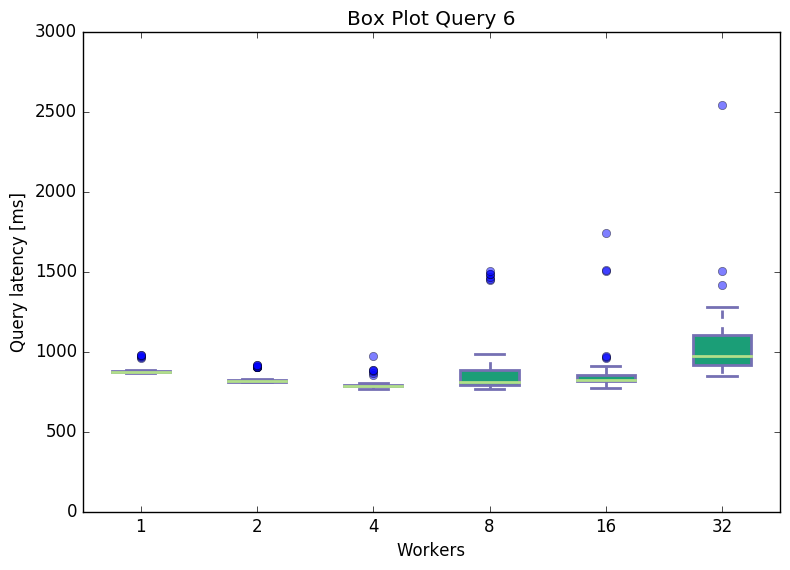
\includegraphics[width=\textwidth]{boxesfl/q6}
    \captionof{figure}{Large Fattree}
  \end{minipage}
  \hfill
  \begin{minipage}[b]{0.5\textwidth}
    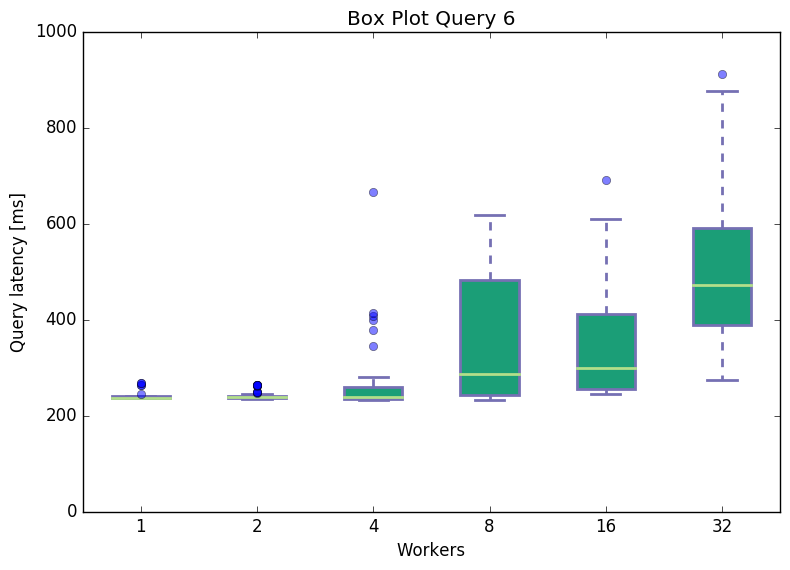
\includegraphics[width=\textwidth]{boxesfs/q6}
    \captionof{figure}{Small Fattree}
  \end{minipage}
\end{figure}
\begin{figure}[!tbp]
  \centering
  \RawFloats
  \begin{minipage}[b]{0.5\textwidth}
    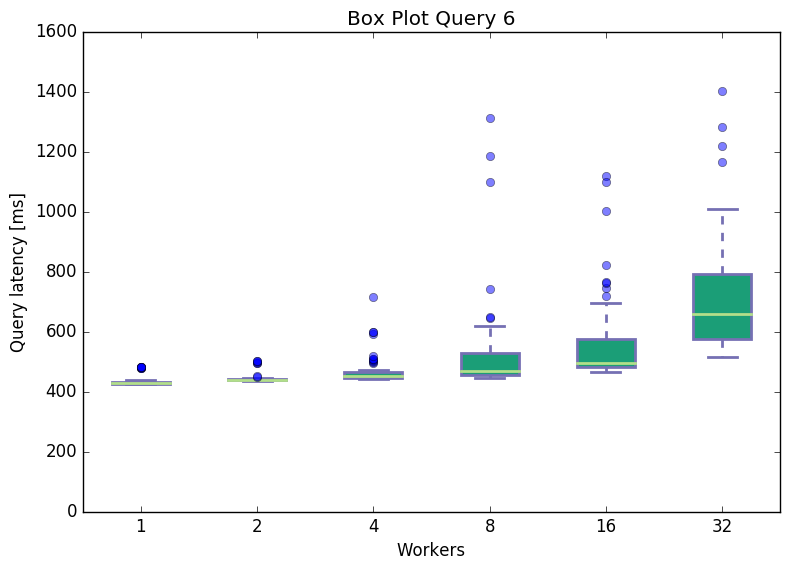
\includegraphics[width=\textwidth]{boxesjl/q6}
    \captionof{figure}{Large Jellyfish}
  \end{minipage}
  \hfill
  \begin{minipage}[b]{0.5\textwidth}
    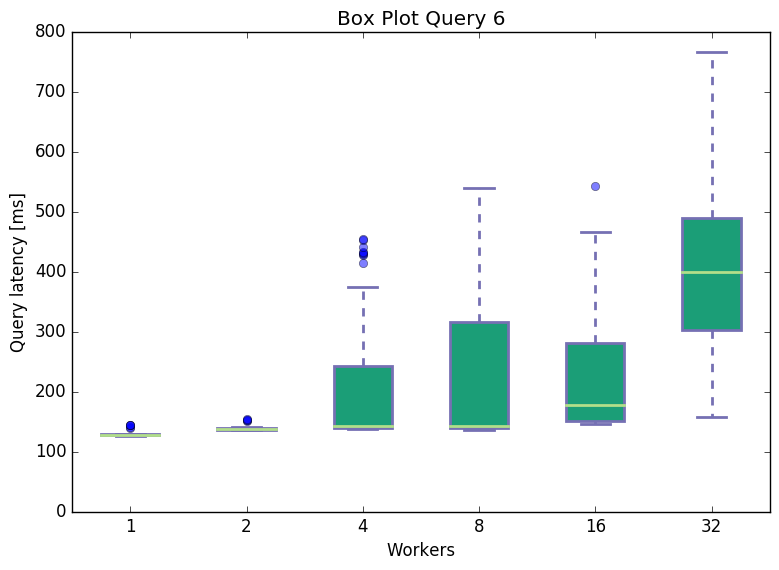
\includegraphics[width=\textwidth]{boxesjs/q6}
    \captionof{figure}{Small Jellyfish}
  \end{minipage}
\end{figure}
\clearpage
\section{Query7}
\begin{verbatim}
SELECT v.name WHERE (u WITH position = 'access')
 -[e with weight  < 2]-> (v WITH position = 'distribution')
 -[f with weight  < 2]-> (w WITH position = 'core')
 -[g with weight  < 2]-> (x WITH position = 'distribution')\end{verbatim}
\textbf{Peak Memory: 2'210'824 kb}\\
\textbf{Result size: 49'956}\\
6 Joins and 7 Selections. This is probably the most interesting result. We add two more joins to the query, but we restrict the number of edges used in all the joins dramatically. This consequently leads to a surprisingly low evaluation time, almost on the level as query 5. This demonstrates how big the impact of the joins is for the evaluation time.\\\\
\textbf{Dataflow}
\begin{figure}[H]
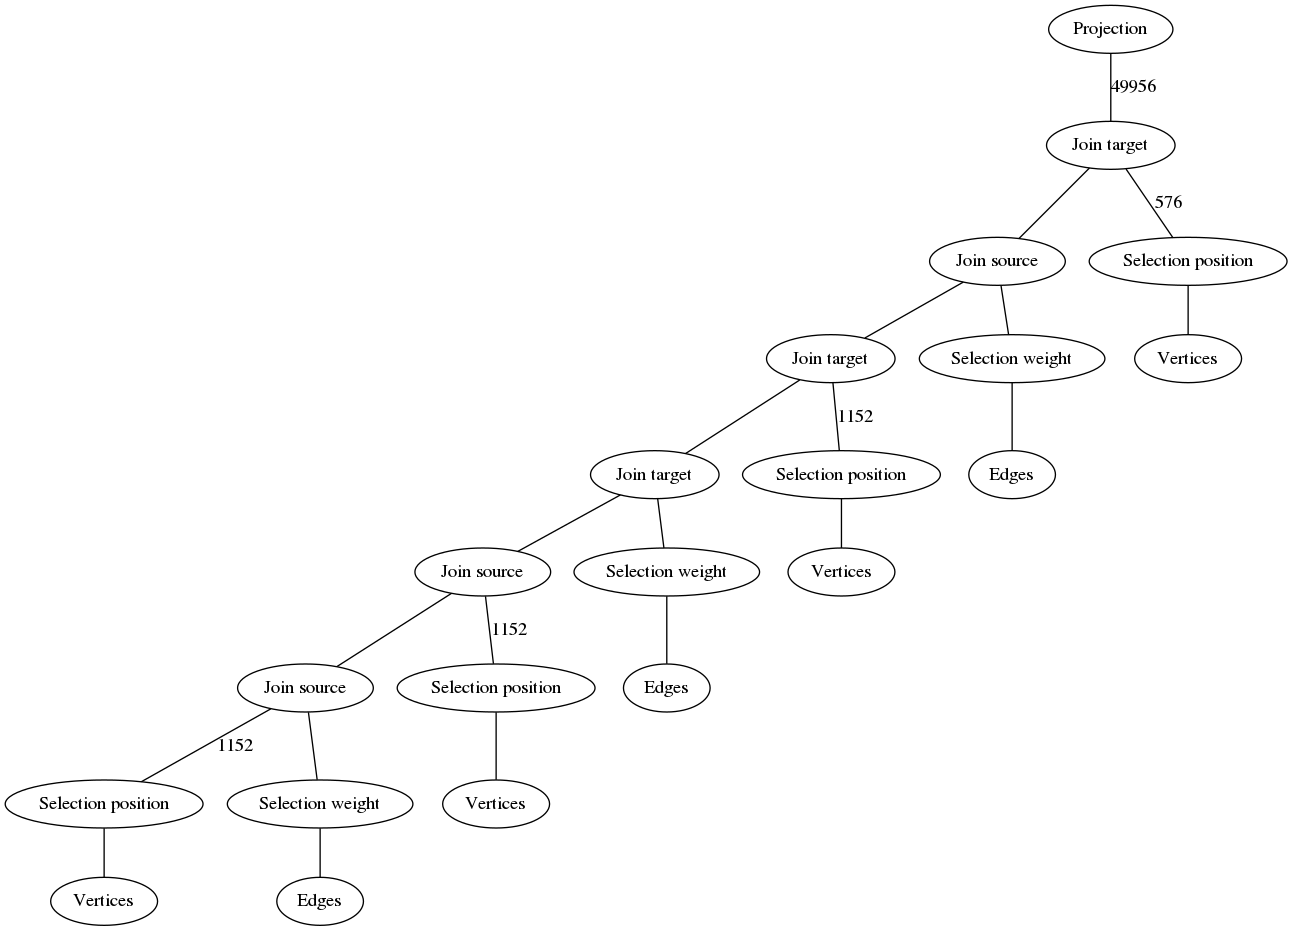
\includegraphics[width=0.8\textwidth]{graph7}
\caption{Dataflow Query7}
\end{figure}
\clearpage
\begin{figure}[!tbp]
  \centering
  \RawFloats
  \begin{minipage}[b]{0.5\textwidth}
    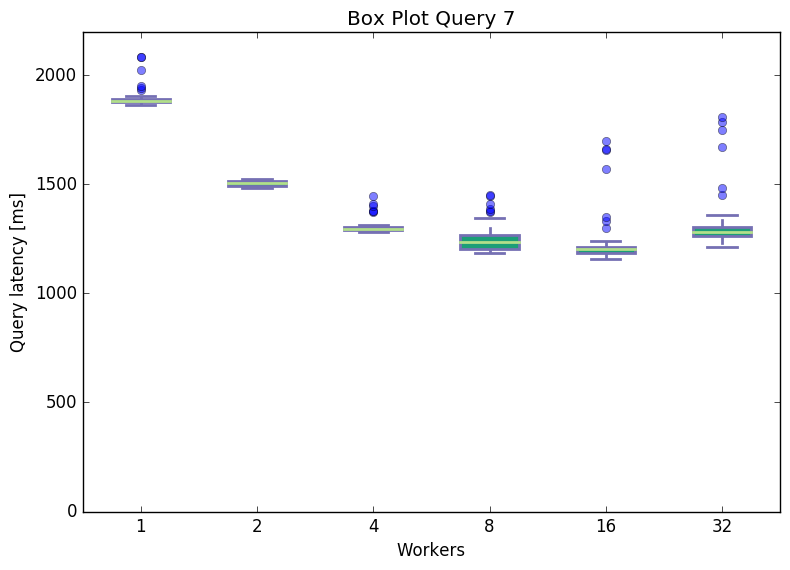
\includegraphics[width=\textwidth]{boxesfl/q7}
    \captionof{figure}{Large Fattree}
  \end{minipage}
  \hfill
  \begin{minipage}[b]{0.5\textwidth}
    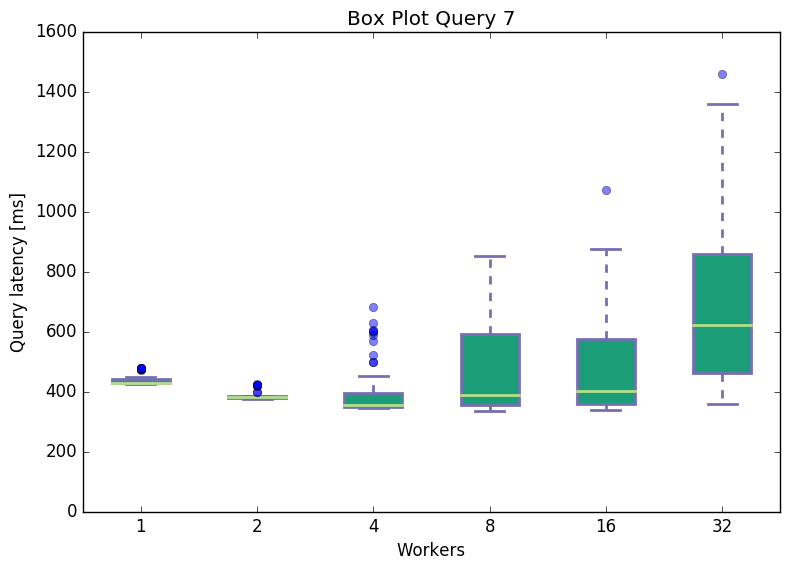
\includegraphics[width=\textwidth]{boxesfs/q7}
    \captionof{figure}{Small Fattree}
  \end{minipage}
\end{figure}
\begin{figure}[!tbp]
  \centering
  \RawFloats
  \begin{minipage}[b]{0.5\textwidth}
    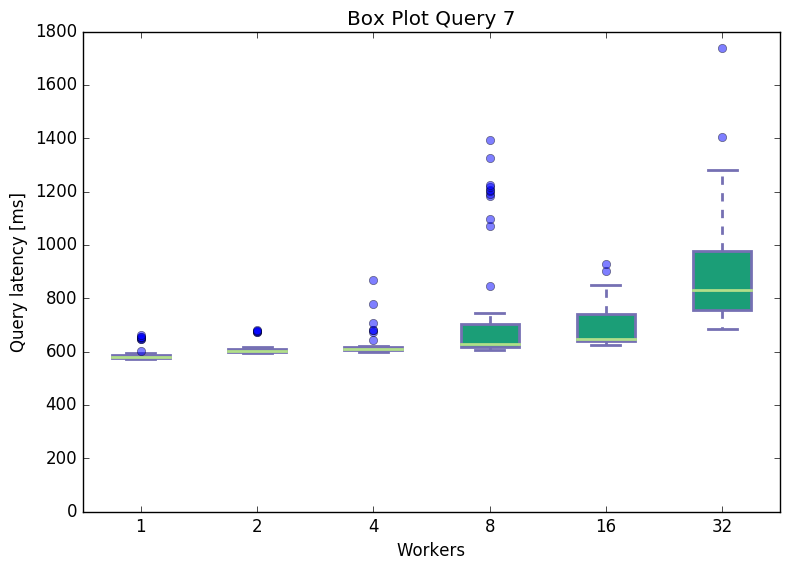
\includegraphics[width=\textwidth]{boxesjl/q7}
    \captionof{figure}{Large Jellyfish}
  \end{minipage}
  \hfill
  \begin{minipage}[b]{0.5\textwidth}
    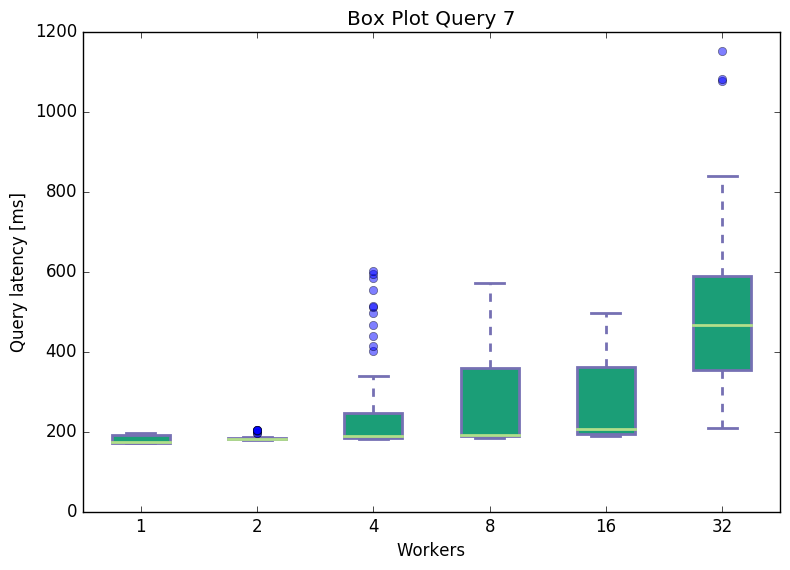
\includegraphics[width=\textwidth]{boxesjs/q7}
    \captionof{figure}{Small Jellyfish}
  \end{minipage}
\end{figure}
\clearpage


\end{document}